% Software Overview
% MIT License
%
% Copyright (c) 2026 HumberASV
% Copyright (c) 2026 Carson Fujita
%
% Permission is hereby granted, free of charge, to any person obtaining a copy
% of this software and associated documentation files (the "Software"), to deal
% in the Software without restriction, including without limitation the rights
% to use, copy, modify, merge, publish, distribute, sublicense, and/or sell
% copies of the Software, and to permit persons to whom the Software is
% furnished to do so, subject to the following conditions:
%
% The above copyright notice and this permission notice shall be included in all
% copies or substantial portions of the Software.
%
% THE SOFTWARE IS PROVIDED "AS IS", WITHOUT WARRANTY OF ANY KIND, EXPRESS OR
% IMPLIED, INCLUDING BUT NOT LIMITED TO THE WARRANTIES OF MERCHANTABILITY,
% FITNESS FOR A PARTICULAR PURPOSE AND NONINFRINGEMENT. IN NO EVENT SHALL THE
% AUTHORS OR COPYRIGHT HOLDERS BE LIABLE FOR ANY CLAIM, DAMAGES OR OTHER
% LIABILITY, WHETHER IN AN ACTION OF CONTRACT, TORT OR OTHERWISE, ARISING FROM,
% OUT OF OR IN CONNECTION WITH THE SOFTWARE OR THE USE OR OTHER DEALINGS IN THE
% SOFTWARE.

% Section is expected to follow GUI and not Development, but it can be moved if needed.
\section{GUI Development}

Following \hyperref[sec:basestation-previous-implementation]{the previous implementation of the base station}, we have decided to implement with Flask instead of Django for the web server component of the base station.
Flask is a lightweight web framework\autocite{FLASK} which can also scale and handle the \hyperref[sec:basestation-user-needs]{user needs} of our web client application without the overhead of Django's features that we do not require.

We will use flask to create a web server that will handle the following tasks:

\begin{itemize}
    \item create an API for handling security tokens (under \hyperref[itm:fr-webclient-token]{FR-21} and \hyperref[itm:fr-webclient-admin]{FR-22}) 
    \item to serve the web client application to users.
    \item stream the video feed from process 2.8 (Telemetry) in Figure \ref{fig:base-station-diagram} to the web client application.
    \item stream telemetry data from process 2.8 (Telemetry) in Figure \ref{fig:base-station-diagram} to the web client application for visualization.
\end{itemize}

\subsection{Streaming Video and Telemetry Data}

\subsection{Security Token Management}
Before serving the \textit{/client} page, the website host verifies that telemetry and video streams from the ASV are being received. 
If the streams are unavailable, the site displays an error page and access to the web client is withheld until data reception resumes. 
When streams are available, the host prompts the user to enter a token (see the ``Get Login page'' step in the sequence diagram, Figure \ref{fig:seq-connection}). 
The submitted token is sanitized and checked against the database (D1 in Figure \ref{fig:base-station-diagram} and Figure \ref{fig:seq-connection}); 
a valid token grants access to the web client and its live telemetry and video, while an invalid token results in an error page denying access. 
This behavior implements the token API (\hyperref[itm:fr-webclient-token]{FR-21}) and the admin token management features (\hyperref[itm:fr-webclient-admin]{FR-22}), 
ensuring only authorized users may view ASV data and video feeds.

\begin{figure}[H]
    \centering
    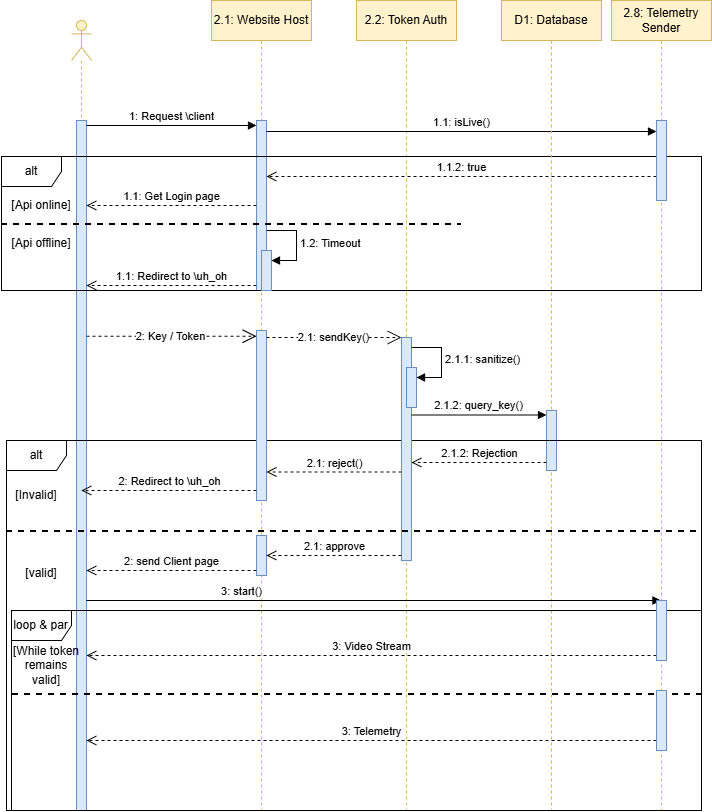
\includegraphics[width=0.8\textwidth]{./images/GUI/sequence-connection.png}
    \caption{Sequence Diagram for User Connection to Web Client}
    \label{fig:seq-connection}
\end{figure}

\notebox{Technical users, such as the Humber ASV team, will have access to an admin webpage within the web client application that allows them to create, revoke, and expire tokens as needed to maintain security.}
